% !Mode:: "TeX:UTF-8"

\chapter{基于深度嵌入卷积聚类方法的地海杂波无监督分类}
\label{sec:decc}
\section{引言}
由于天波雷达地海杂波频谱数据量大,进行人工标定的成本十分昂贵,且当雷达工作频率变化导致数据的相干积累点数变化时需要重新标定数据对网络进行训练。无监督学习(又称聚类)算法是解决该问题的一个很好的思路,但是传统的聚类算法的性能受数据维数以及样本数据量的影响,会产生维数灾难的问题。为了克服这个困难,研究者一般选择将高维度的数据映射到低维,然后将嵌入数据聚类到这个新的子空间中\ucite{roth2004feature}的方法,该方法分为特征学习和聚类这两个割裂的阶段,影响了最终的聚类精度。

本章提出了一种新的联合解决共同完成特征学习和聚类的算法,深度嵌入卷积聚类方法(Deep Embedding Convolution Clustering, DECC)。通过利用卷积自编码器进行特征提取,可以充分挖掘数据的局部信息,设计了新的损失函数用于同时更新网络和聚类中心参数。
% 聚类方法如今已经在各个领域得到了广泛应用
% 对数据集规模较大的情形,有一些研究只选择数据集的一个子集来加速聚类过程\ucite{shinnou2008spectral}。
% 为了解决计算复杂度的问题,以往的研究往往首先
% 这类算法可以分为两个阶段:特征学习和聚类,其主要思想是向目标函数中添加表征稀疏性或者是图形约束的先验知识进行训练学习\ucite{tian2014learning}。

% 特征学习指的是一类试图利用一组通常稀疏的特征向量来描述一个数据集的学习方法。
% 在实践中,有很多不同的算法可以进行特征学习,包括自编码器、高斯混合模型(Gaussian Mixture Model, GMM)和受限玻尔兹曼机。
% 这些方法主要学习一个近似局部滤波器字典\ucite{coates2011analysis},例如用于自然图像的Gabor类边缘滤波器或者用于MNIST数字数据集的书写笔划。

本章安排如下: \ref{sec:cae}节对卷积自编码网络进行了介绍,\ref{sec:decc_method}节构建了本章利用的深度嵌入卷积聚类器,通过利用卷积自编码器对输入地海杂波进行重构,然后利用本章提出的聚类损失函数进行训练,最终获得聚类结果,\ref{sec:decc_experiment}节利用实际数据对本章提出的算法性能进行了分析讨论,\ref{sec:decc_summary}节进行本章总结。

\section{卷积自编码网络}
\label{sec:cae}
\subsection{自编码器}

自编码器是一种利用隐层重构输入的神经网络。其模型如图\ref{fig:ae}所示,它由编码器(Encoder)和解码器(Decoder)两部分组成,本质上是对输入信号的某种变换。
\begin{figure}[hbt]
	\centering
	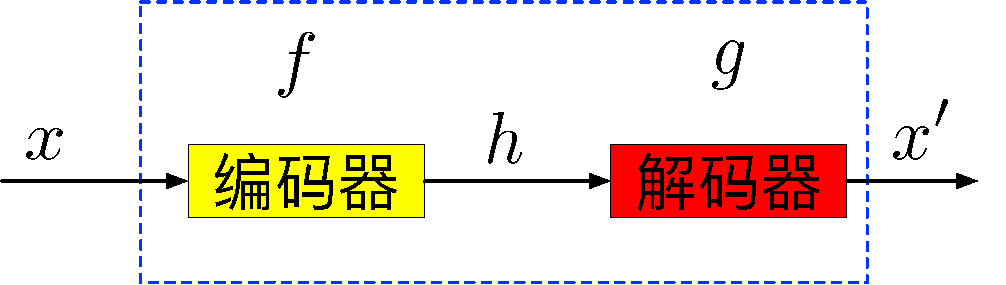
\includegraphics[width=9cm]{figures/AE/ae}
	\caption{自编码器模型}
	\label{fig:ae}
\end{figure}
对一组具有$N$个输入向量的给定输入数据集,
编码器将第$i$个输入信号$x^{(i)}\in\mathbb{R}^{d_x}$编码到某个隐层的表示$h^{(j)}\in\mathbb{R}^{d_h}$,$d_x$和$d_h$分别为输入表示和隐层表示的维数,然后解码器再将$h^{(j)}$解码为输出$x'^{(i)}\in\mathbb{R}^{d_x}$。通过最小化$x^{(i)}$与$x'^{(i)}$之间的差距,可以训练得到一个用来重构输入特征的映射。
编码和解码公式如下:
\begin{align}
	h^{(j)}_n &= f(b_n+\sum_{m=1}^{d_x}w_{mn}x^{(i)}_m), \\
	x'^{(i)}_m &= f(b'_m+\sum_{n=1}^{d_h}w'_{mn}h^{(j)}_n),
\end{align}
其中,$f$是激活函数函数,${W}=[w_{mn}]$和${W}'=[w'_{mn}]$分别为编码器和解码器的权重矩阵,${b}=[b_n]$和${b'}=[b'_m]$分别为编码器和解码器的偏置向量。

在此基础上,国内外广大学者对自编码器进行了各种改进,提出了可以学习输入空间中扰动不变的特征的压缩自编码器\ucite{rifai2011contractive}、
利用高效的变分方法进行训练和生成推理的变分自编码器\ucite{kingma2013auto}
以及可以基于连续的数据流在运行中添加或合并隐层单元的在线增量自编码器\ucite{zhou2012online}。

\subsection{卷积自编码器}
传统的自编码网络只有一个隐层,只能学习出一种特征变化,但是图\ref{fig:sae}所示的堆栈自编码器(Stacked Autoencoders, SAE)在一定程度上解决了这个问题。
% 于是Bengio\ucite{bengio2007greedy}等人在2007年的仿照stacked RBM构成的DBN,提出堆栈自编码器(Stacked Autoencoders, SAE),为非监督学习在深度网络的应用又增加了一种重要的思路方法。%--查重去掉
% 堆栈自编码器模型可以参看图\ref{fig:sae},其通过逐层非监督学习的预训练,也即逐层初始化(Layer-wise Pre-training),来初始化深度网络的参数,替代传统的随机初始化的方法。预训练完毕后,利用训练参数,再进行监督学习训练。%--查重去掉
\begin{figure}[hbt]
	\centering
	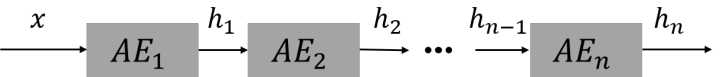
\includegraphics[width=9cm]{figures/AE/sae}
	\caption{堆栈自编码器模型}
	\label{fig:sae}
\end{figure}

全连接自编码器和深度自编码器都忽略了数据的局部结构信息。
这在处理实际大小的输入时不仅是一个问题,而且在参数中引入冗余,迫使每个特征是全局的。
然而,在视觉和对象识别领域最成功的模型\ucite{lowe1999object}均主要利用了在整个输入空间发生重复的局部特征。
基于此,文献\cite{masci2011stacked}提出了一种卷积自编码器(Convolutional Autoencoders, CAE)。
卷积自编码器不同于传统的自编码器,它们的权重在输入向量中的所有位置之间共享,从而可以保持空间局部性。
因此重构结果是隐层局部特征的线性组合。
从结构的角度看,CAE类似于SAE,但是将SAE中的全连接神经网络变为了卷积神经网络。
参考第\ref{sec:network}章\equref{equ:shared_weight},设输入为$x$,第$k$个特征映射的隐层表示则由\equref{equ:cae1}给出:
\begin{equation}
	h^k=f(x*W^k+b^k)
	\label{equ:cae1}
\end{equation}
其中$b^k$是全局共享的偏置,$f$是激活函数,$*$表示卷积操作。
% 为了使得每个滤波器专注于整个输入空间的一种特征,另一方面如果每个数据点一个偏置将引入太多的自由度,所以对每一个隐层使用相同的偏置。
\equref{equ:cae1}生成的隐层表示是输入$x$在低维空间中的编码,
由于自编码器的目标是从所生成的特征映射重构输入$x$,因此需要相应的解码操作。卷积自编码器是完全卷积网络,因此解码操作也是一个卷积操作,一般称为反卷积操作(Deconvolution)或者转置卷积(Transposed Convolution)。

隐层表示$h^k$被用来作为解码器的输入,为了使得解码器的输出和原始的输入数据具有相同的结构,解码器反卷积的超参数由编码器的结构确定,
因此,解码器的重构过程的计算公式为:
\begin{equation}
	x'^k=f(\sum_{k \in H}h^k * \tilde{W}^k + b'^k).
	\label{equ:cae2}
\end{equation}
同样的,每一个输入通道只有一个偏置$b'^k$,$H$表示所有特征图的集合,
$\tilde{W}$ 表示在两个维度上进行翻转操作后的权重。

正如第\ref{sec:network}章介绍,一般的分层网络特别是卷积神经网络,通常引入池化层来获得平移不变性。因此本章的卷积自编码器在编码器阶段添加了池化层,相应的在解码器阶段需要添加上采样来进行处理,如图\ref{fig:unpool}所示。
\begin{figure}[hbt]
	\centering
	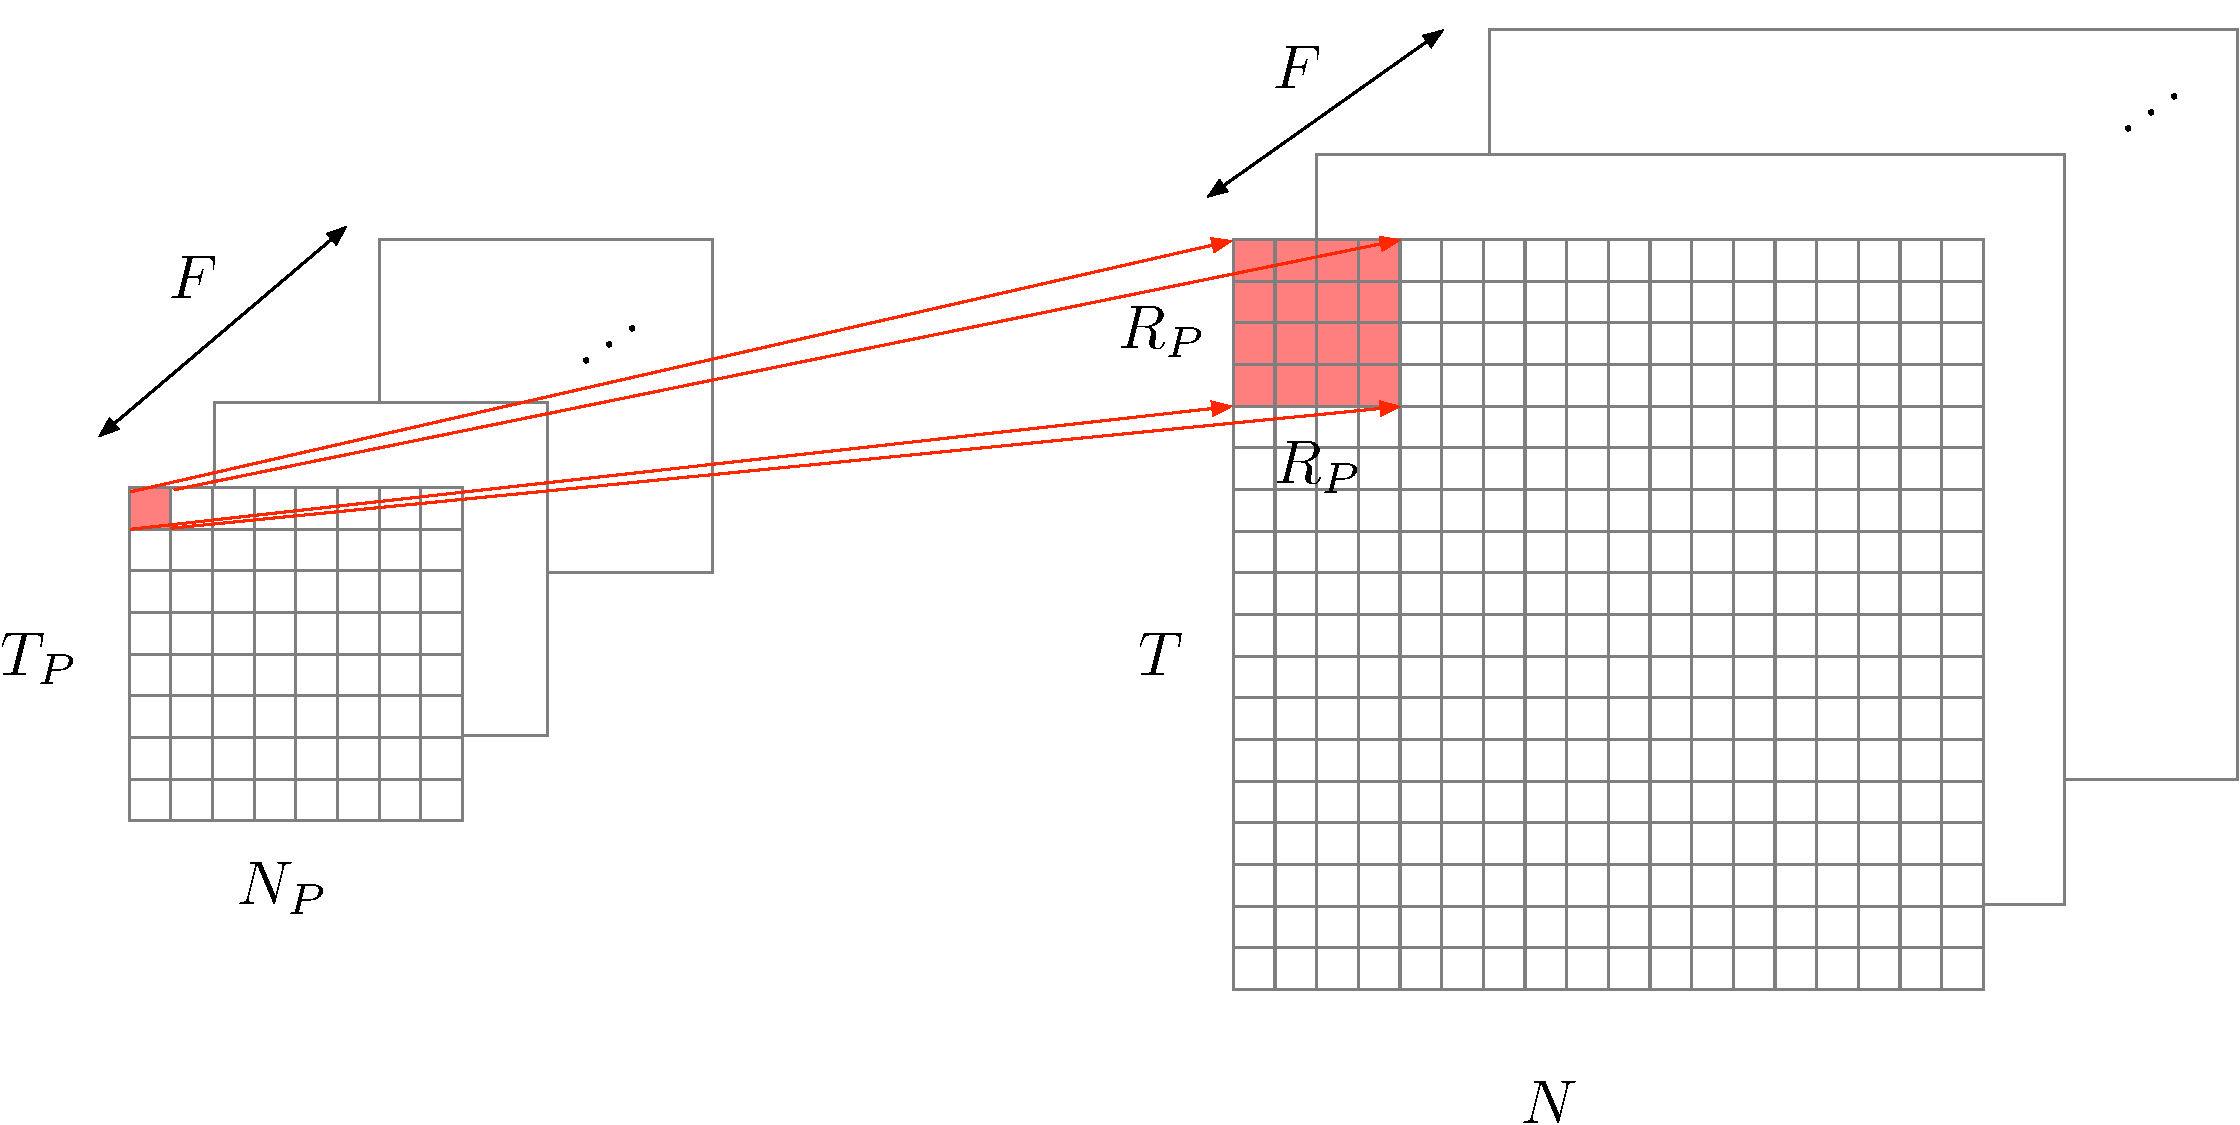
\includegraphics[width=13.5cm]{figures/AE/unpool}
	\caption{上采样示意图}
	\label{fig:unpool}
\end{figure}

模型参数$\Theta=\{{W},{b},{b'}\}$通过最小化其损失函数进行求取,一般利用均方误差损失函数(mean squared error, MSE):
\begin{align}
	\mathscr{L} &= \frac{1}{N}\sum_{i=1}^N||x_i-x_i'||_2^2, \label{equ:mse_loss}\\
	\theta^* &= arg\min\limits_{\theta} \mathscr{L}.  \label{equ:mse}
\end{align}
就像标准的神经网络一样,反向传播算法被用来计算相对于参数的误差函数的梯度,则可以得到:
\begin{equation}
	\frac{\partial \mathscr{L}}{\partial W^k}=x * \Delta h ^k+\tilde{h}^k * \Delta x',
\end{equation}
$\Delta h$ 和 $\Delta x'$分别是隐层状态和重构结果的变化量,然后可以使用随机梯度下降(SGD)等基于梯度的优化算法来更新权重。

相比于传统自编码器,卷积自编码器更有利于学习数据的局部结构,避免特征空间的失真。
虽然卷积自编码器的过完备隐层表示使得其学习比标准自编码器更难,但是可以通过添加池化层加强其稀疏性来在一定程度上降低计算量。

\section{深度嵌入卷积聚类方法}
\label{sec:decc_method}
深层嵌入聚类算法\ucite{xie2016unsupervised}提供了一种以无监督的方式同时学习特征表示与聚类的思路,提高了聚类算法的性能和鲁棒性。
但是,该算法用于特征提取的堆栈自编码器需要逐层预训练,然后以端到端训练的方式进行微调。当层次增加时,预训练过程所需时间会急剧增加。此外,堆栈自编码器是建立在全连接网络上,对处理局部信息是无效的。
因此本章在此基础上利用卷积自编码器代替传统的堆栈自编码器并设计了新的损失函数,提出了深度嵌入卷积聚类方法(Deep Embedding Convolution Clustering, DECC)。

\subsection{深度嵌入卷积聚类方法结构}
首先进行问题描述,假设需要将$N$个样本$X=[x_1,\dots,x_N]$聚为$K$个类别,其聚类中心点为$\mu_1,\dots,\mu_K$,其中每一个样本$x_i\in \mathbb{R}^{d_x}$,由于当样本维数增大时会会产生维数灾难的问题,因此需要引入一个嵌入函数$\varphi_W: X \rightarrow Z$,可以将原始样本映射到嵌入子空间$Z=[z_1,\dots,z_N]$,其中$z_i\in \mathbb{R}^{d_z}$的维数远小于原始样本的维数,也即$d_z<<d_x$。
然后,利用K-均值聚类算法,将子空间$Z$进行聚类,得到初始聚类中心${\mu_k}$。

本章利用卷积自编码器作为嵌入函数对原始样本进行降维,其结构如图 \ref{fig:cae} 所示。
通过三次卷积操作充分提取输入样本的特征,同时在所有层添加ReLU激活函数,并且在编码器后以相反的顺序放置反卷积解码器。在编码器与解码器中间添加嵌入层(图\ref{fig:cae}中黄色标记的全连接层),该层的结果被用于进行聚类操作。DECC的结构如图 \ref{fig:decc} 所示。
\begin{figure}[hbt]
	\centering
	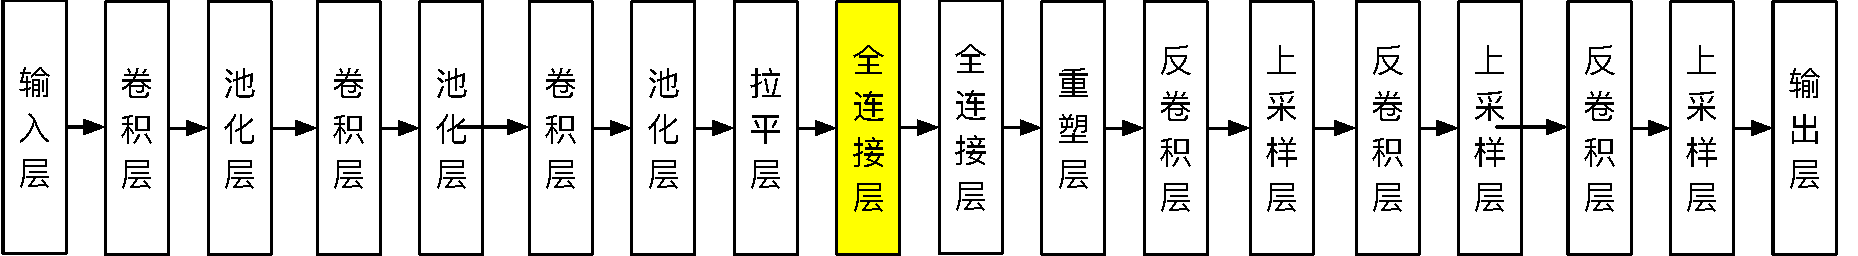
\includegraphics[width=13.5cm]{figures/AE/cae}
	\caption{卷积自编码器结构图}
	\label{fig:cae}
\end{figure}

\begin{figure}[hbt]
	\centering
	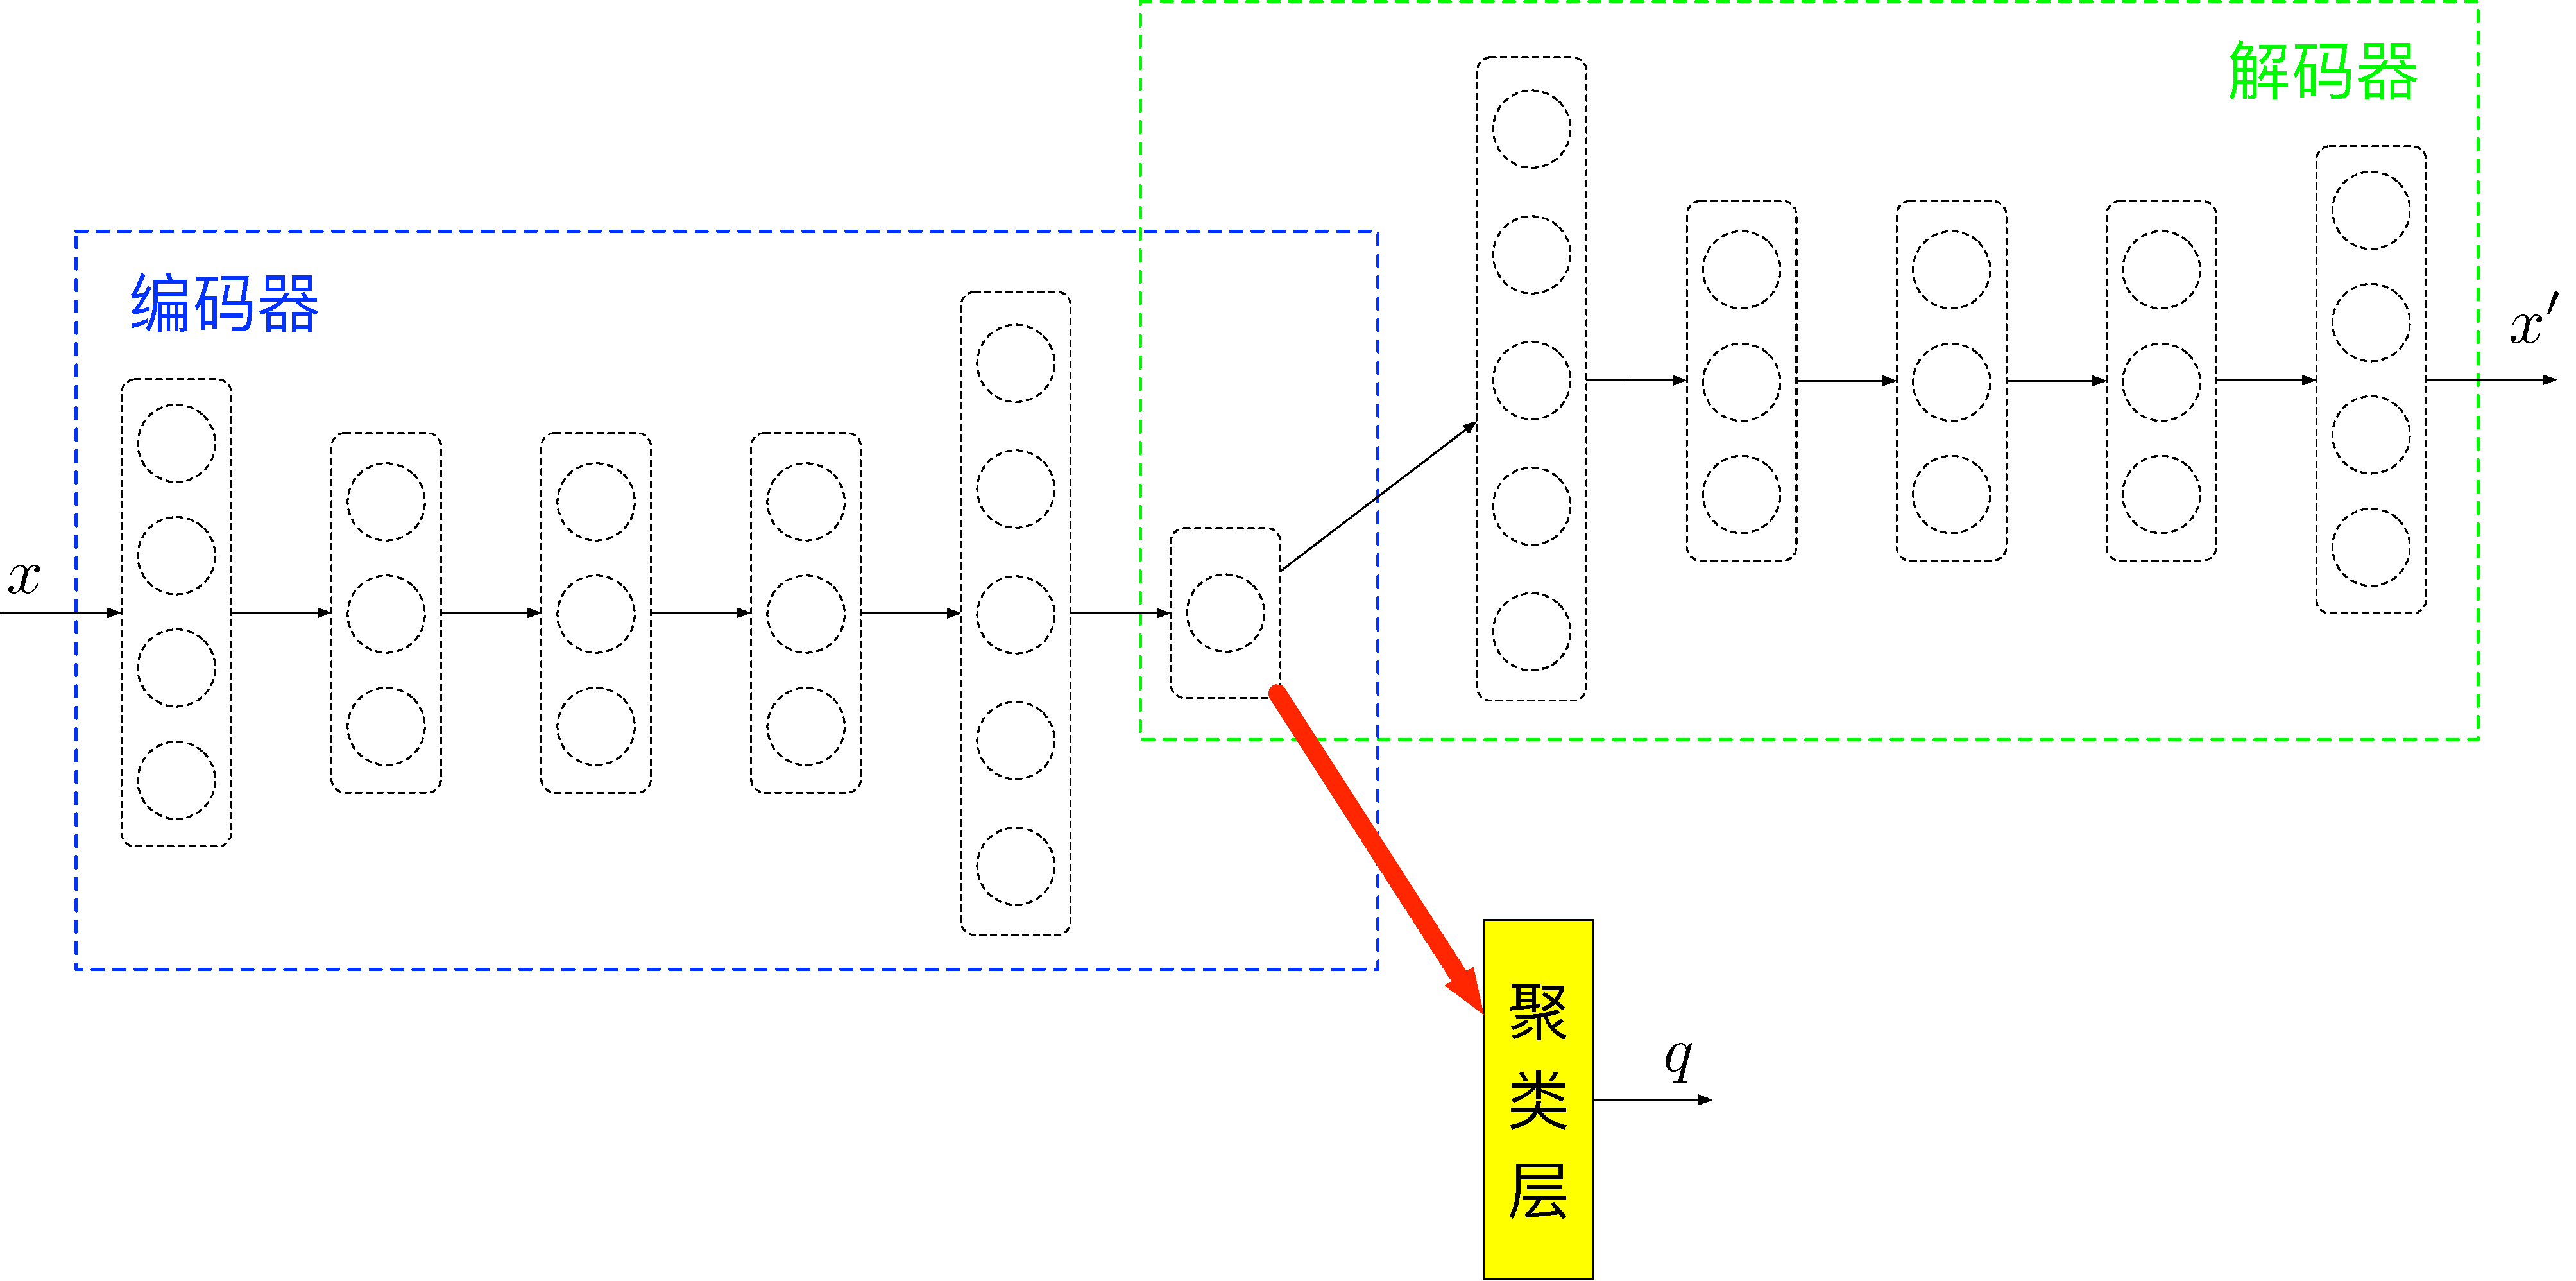
\includegraphics[width=13.5cm]{figures/AE/decc}
	\caption{深度嵌入卷积自编码器结构图}
	\label{fig:decc}
\end{figure}

\subsection{KL散度聚类方法}
文献\cite{maaten2008visualizing}利用学生t分布来衡量嵌入点$z_i$与聚类中心点$\mu_k$的相似度:
\begin{equation}
p_{ik}=\frac{(1+||z_i-\mu_k||^2/\alpha)^{-\frac{\alpha+1}{2}}}{\sum_{k'}(1+||z_i-\mu_k||^2/\alpha)^{-\frac{\alpha+1}{2}}},
	\label{equ:p}
\end{equation}
其中,$\alpha$为学生t分布的自由度,$p_{ik}$可以看作样本$i$到类别$k$的概率。

为了定义本章的聚类目标函数,可以使用辅助目标变量(auxiliary target variable)$Q$来迭代地改进模型预测。首先用Kullback-Leibler(KL)散度来减小模型预测$P$和目标分布$Q$之间的距离。
\begin{equation}
	\mathscr{L}_{kld}=KL(Q||P)=\frac{1}{N}\sum_{i=1}^{N}\sum_{k=1}^{K}q_{ik}\log{\frac{q_{ik}}{p_{ik}}},
	\label{equ:kldfirst}
\end{equation}
根据文献\cite{xie2016unsupervised},目标分布$Q$的定义如下:
\begin{equation}
	q_{ik}=\frac{p_{ik}^2/f_k}{\sum_k(p_{ik}^2/f_k)},
	\label{equ:traget_distribution}
\end{equation}
其中$f_k$的定义为
\begin{equation}
	f_k=\sum_iq_{ik}
\end{equation}

\equref{equ:mse}给出了自编码器重构的损失函数,故最终的损失函数为:
\begin{equation}
	\mathscr{L}=\mathscr{L}_{mse}+\beta \mathscr{L}_{kld},
	\label{equ:l_last}
\end{equation}
其中,$\beta > 0$为调节两部分损失函数权重的参数。

\subsection{学习算法}
本章利用随机梯度下降和反向传播对\equref{equ:l_last}中的损失函数进行学习。根据上一节的描述可知,总共有三类参数需要学习:卷积自编码器的权重、聚类中心以及目标分布$Q$。
\subsubsection{更新卷积自编码器的权重和聚类中心}
对一个给定的目标分布$Q$,那么聚类损失$\mathscr{L}_{kld}$相对于嵌入点$z_i$和聚类中心点$\mu_k$的梯度计算公式如下:
\begin{align}
	\frac{\partial \mathscr{L}_{kld}}{\partial z_i} &= 2\sum_{k=1}^K(1+||z_i-\mu_k||^2)^{-1}(q_{ik}-p_{ik})(z_i-\mu_k), \\
	\frac{\partial \mathscr{L}_{kld}}{\partial \mu_k} &= 2\sum_{i=1}^N(1+||z_i-\mu_k||^2)^{-1}(p_{ik}-q_{ik})(z_i-\mu_k). \\
\end{align}
那么对于一个小的批次$m$和学习率$\lambda$,$\mu_k$的更新为:
\begin{equation}
	\mu_k=\mu_k-\frac{\lambda}{m}\sum_{i=1}^m{\frac{\partial \mathscr{L}_{kld}}{\partial \mu_k}}.
\end{equation}
编码器的权重更新为:
\begin{equation}
	W=W-\frac{\lambda}{m}\sum_{i=1}^m(\frac{\partial \mathscr{L}_{mse}}{\partial W} + \beta \frac{\partial \mathscr{L}_{kld}}{\partial W}).
	\label{equ:encoder_update}
\end{equation}
解码器的权重更新为:
\begin{equation}
	W'=W'-\frac{\lambda}{m}\sum_{i=1}^m{\frac{\partial \mathscr{L}_{mse}}{\partial W'}}.
\end{equation}
\subsubsection{更新目标分布}
根据\equref{equ:traget_distribution}可知,目标分布$Q$依赖于先验的软指派(soft assignment)$P$。因此,为了提升结果的鲁棒性,本章利用全部嵌入点每隔$T$次迭代对目标分布进行更新,其更新主要利用\equref{equ:p}和\equref{equ:traget_distribution}。并且每次完成更新后,重新计算样本$x_i$的指派:
\begin{equation}
	s_i=arg \max \limits_k p_{ik}
	\label{equ:assign}
\end{equation}
当相邻两次更新的指派变化小于一个阈值$\delta$时,停止迭代,那么则可以得到整个算法流程图。
% \\[420pt]
\begin{algorithm}[H]
	\caption{DECC 算法学习过程}
	\begin{algorithmic}[1] %每行显示行号
		\Require 训练样本$X$,聚类结果个数$K$,最大迭代次数$iter_{max}$,目标分布更新间隔$T$,初始目标参数$\theta$,学习率$\eta$
		\Ensure 卷积自编码器编码器的权重$W$和解码器的权重$W'$,聚类中心$\mu$,指派标签$s$
		\State 初始化迭代次数$iter=1$
		\State 只利用重构损失函数对卷积自编码器进行训练,获得初始权重$W$和$W'$
		\State 利用K-均值聚类算法获得初始聚类中心$\mu$
		\While{$iter < iter_{max}$}
			\If{iter mod T = 0}
				\State 计算所有嵌入点 $z_i=\varphi_W(x_i),i=1,\dots,N$
				\State 将\equref{equ:p}代入\equref{equ:traget_distribution}更新目标分布 $Q$
				\State 保存上一次指派$s_{last}=s$
				\State 计算新的指派 $s_i=arg \max \limits_k p_{ik}, i= 1,\dots,N$
				\If{$sum(s_{last} \neq s) / N < \delta $}
					\State 停止学习
				\EndIf
			\EndIf
			\State 从训练集中获取$m$ 个采样样本 $\{x^{(1)},\dots,x^{(m)}\}$ ,其中$m$ 为批处理中一批样本的个数。
			\State 更新聚类中心$\mu_k=\mu_k-\frac{\lambda}{m}\sum_{i=1}^m{\frac{\partial \mathscr{L}_{kld}}{\partial \mu_k}}$
			\State 更新编码器权重 $W=W-\frac{\lambda}{m}\sum_{i=1}^m(\frac{\partial \mathscr{L}_{mse}}{\partial W} + \beta \frac{\partial \mathscr{L}_{kld}}{\partial W})$
			\State 更新解码器权重 $W'=W'-\frac{\lambda}{m}\sum_{i=1}^m{\frac{\partial \mathscr{L}_{mse}}{\partial W'}}$
		\EndWhile
	\end{algorithmic}
\end{algorithm}
\section{仿真验证}
\label{sec:decc_experiment}
% \subsection{算法设置}
本章利用第\ref{sec:othr}章中组C的训练数据用于本章的实验,考虑到地海杂波在时间与空间上的连续性,本章选取了相邻3帧,相邻9个单元共27个单元的杂波信号将其进行组合,并进行随机重排复制得到一个$128\times 128$的二维数据,其示意图参看图 \ref{fig:unsurpvised_data}。
\begin{figure}[hbt]
	\centering
	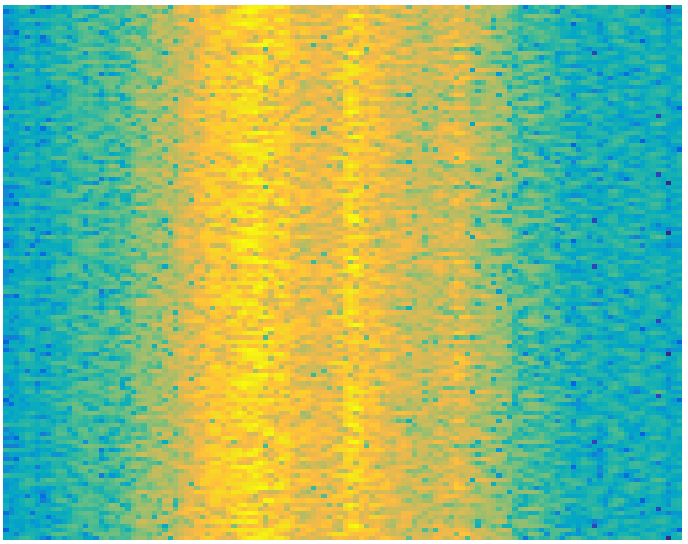
\includegraphics[width=6.67cm]{figures/AE/unsurpvised_data}
	\caption{输入样本示意图}
	\label{fig:unsurpvised_data}
\end{figure}

本章根据图\ref{fig:cae}设计的卷积自编码器进行特征的降维,该部分进行30次迭代,学习方法为Adam,嵌入层为10维,也即利用10维的特征向量对原始输入信号进行表示。
然后根据此特征向量,随机进行20次K-均值算法,然后从中选取最优结果作为起始的聚类中心点,此也作为本章的一个对比算法。损失函数的权重系数$\beta = 0.1$,学生t分布的自由度$\alpha = 1$。
最终的优化问题通过小批量随机梯度下降和反向传播得到有效解决,其中批长度为256,学习率为0.01。

% \subsection{仿真结果分析}
本章对比了不同算法的无监督聚类精度(ACC)、归一化信息(Normalized Mutual Information, NMI)和调整兰德指数(Adjusted Rand Index, ARI),来比较不同算法的聚类结果的准确率、聚类结果与真实情况的相似程度及每个类内的纯度等信息,实验结果如表\ref{tab:uns}所示。
实验结果证明本章提出的利用深度嵌入卷积算法的正确度相比于K-均值算法有了显著的提高,而添加了重构损失函数后的结果又有了进一步的提高。但是由于卷积运算的计算量比较大以及多个损失函数共同作用导致聚类收敛迭代次数要大于仅利用全连接网络的DEC算法。DECC与DEC的聚类收敛结果的对比,如图\ref{fig:unsurpvised_acc}和\ref{fig:unsurpvised_loss}所示,可以发现DEC算法的收敛速度很快,但是精度不如DECC算法。
\begin{table}[hbt]
	\renewcommand{\arraystretch}{1.3}
	\caption{无监督聚类精度对比表}
	\label{tab:uns}
	\centering\sWuhao
	\begin{tabularx}{\textwidth}{>{\centering\arraybackslash}X>{\centering\arraybackslash}X>{\centering\arraybackslash}X>{\centering\arraybackslash}X>{\centering\arraybackslash}X}
		\toprule
		 方法 & 无监督聚类精度 & 归一化互信息 & 调整兰德指数  \\
		 \midrule
		DEC & $94.88\%$ & 0.73 & 0.81 \\
		CAE + K-均值 & $88.68$ & 0.58 & 0.60  \\
		DECC($\beta=0$) & $95.63\%$ & 0.78 & 0.83 \\
		DECC & $97.85\%$ & 0.86 & 0.92 \\
		 \bottomrule
	\end{tabularx}
\end{table}

\begin{figure}[hbt]
	\centering
	\begin{minipage}{7cm}
		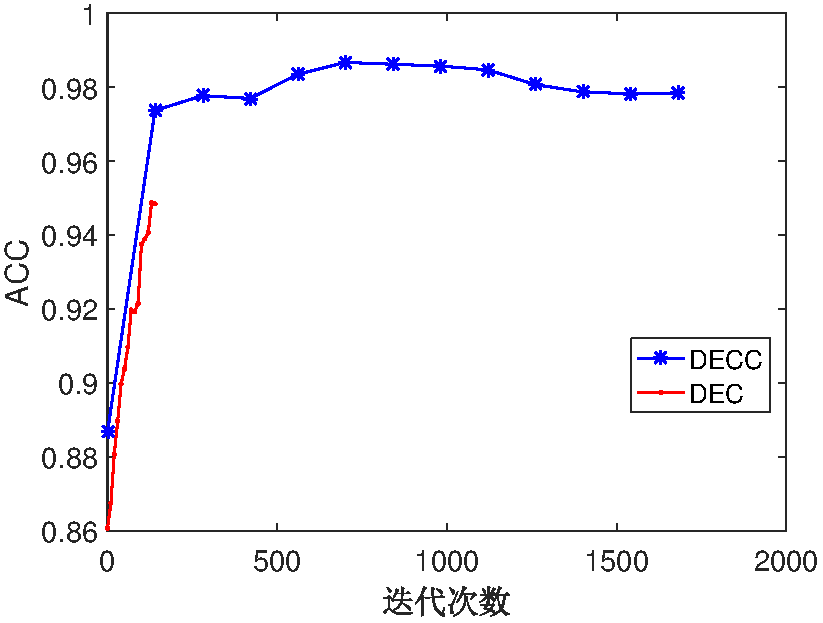
\includegraphics[width=6.67cm]{figures/ae/unsurpvised_acc}
    \caption{DECC与DEC聚类精度对比图}
    \label{fig:unsurpvised_acc}

	\end{minipage}
	\hspace{10pt}
	\begin{minipage}{7cm}
		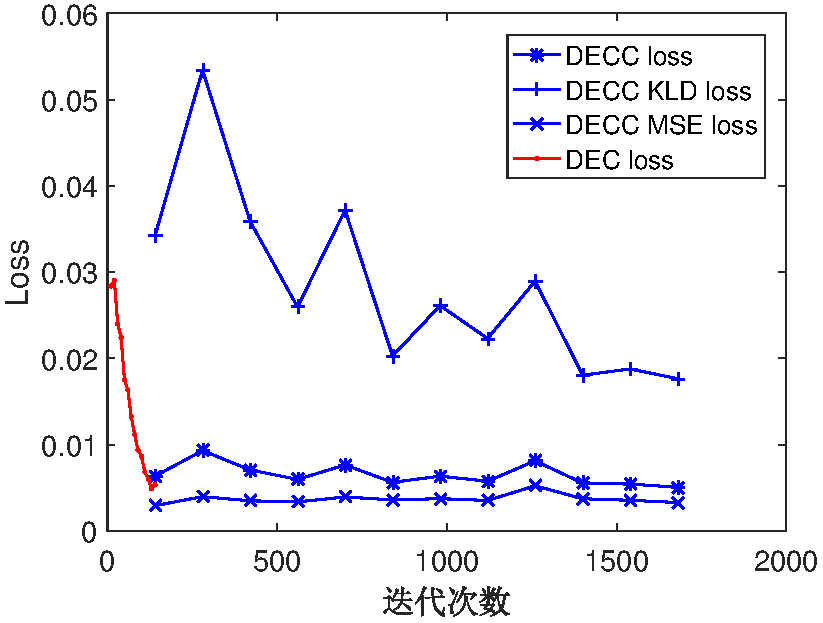
\includegraphics[width=6.67cm]{figures/ae/unsurpvised_loss}
    \caption{DECC与DEC损失函数对比图}
    \label{fig:unsurpvised_loss}

	\end{minipage}

\end{figure}

\section{小结}
\label{sec:decc_summary}
本章结合卷积神经网络与自编码器提出了深度嵌入卷积聚类方法,利用卷积自编码器进行特征提取使得数据的局部信息得以保留,并在损失函数中将KL散度与重构损失两部分结合有效提高了聚类精度。
虽然与有监督学习算法相比,本章的算法精度仍需进一步提高,但是无监督学习的特性克服了大量数据进行标记的成本过高以及部分数据难以人工准确标记的问题。
% 本章的主要贡献如下:
% \begin{itemize}
% 	\item 本章设计了可以以端到端方式训练的卷积自编码器来从未标记的数据中学习特征。通过在地海杂波数据中包含空间、时间信息,通过添加卷积层、卷积转置层和全连接层,设计了好于传统堆栈自编码器的卷积自编码器。
% 	\item 本章提出了深度嵌入卷积聚类算法来自动聚类地海杂波,DECC利用了卷积自编码器提取局部特征的优势。
% 	\item 利用天波超视距雷达的实际地海杂波数据进行了实验,结果验证了深度嵌入卷积聚类算法的有效性。
% \end{itemize}
